\documentclass[conference]{IEEEtran}
\IEEEoverridecommandlockouts
% The preceding line is only needed to identify funding in the first footnote. If that is unneeded, please comment it out.
\usepackage{cite}
\usepackage{amsmath,amssymb,amsfonts}
\usepackage{algorithmic}
\usepackage{graphicx}
\usepackage{url}
\usepackage[utf8]{inputenc}
\usepackage{textcomp}
\usepackage{multirow}
\usepackage{subfig}

\usepackage[english,ngerman,brazilian]{babel}
\def\BibTeX{{\rm B\kern-.05em{\sc i\kern-.025em b}\kern-.08em
    T\kern-.1667em\lower.7ex\hbox{E}\kern-.125emX}}
\begin{document}

\title{PD4 - Segmentação de cor de pele}

\author{\IEEEauthorblockN{Frederico Guth (18/0081641)}
\IEEEauthorblockA{\textit{Tópicos em Sistemas de Computação, ,} \\
\textit{Turma TC - Visão Computacional (PPGI)}\\
\textit{Universidade de Brasília}\\
Brasília, Brasil\\
fredguth@fredguth.com}
}

\maketitle

\begin{abstract}
Detecção de pele lida com o reconhecimento dos
pixels que representam pele em uma dada imagem. Cor é frequentemente usada por ser invariante a orientacao, tamanho e ser
fácil de processar. Neste projeto, detectamos cor de pele usando
tres tipos de classificadores: por limiarizacao, bayesiano simples
e k-nn. Os resultados comparam qualidade da segmentação em
relação ao tempo de execução dos algoritmos. 
\end{abstract}

\begin{IEEEkeywords}
deteção de pele, espaço de cores, K-NN, naive bayesian, threshold-based
\end{IEEEkeywords}

\section{Introdução}

Deteção de pele é o processo de classificação binária de pixels em imagens como sendo \textit{pele} ou \textit{não-pele}. Diversas aplicações de Visão Computacional lidam com interações com humanos e a deteção de pele é tipicamente usada no pré-processamento de imagens para encontrar regiões de interesse. \cite{teo, kolkur, conci}

Cor é o principal fator na deteção de peles; é invariante à orientação e tamanho e rápida de processar. Apesar da variação de tonalidades de peles entre pessoas de diferentes origens e da variação causada pelas condições de luz na obtenção de imagens\cite{kolkur}, já foi observado que a maior variação é de luminosidade, não de tonalidade\cite{teo}. Em imagens com normalização de brilho, a pele humana se agrupa em pequenas regiões de um espaço de cores\cite{yang}.  Assim, o problema de detecção de pele pode ser abordado como um problema de classificação de cores pixel a pixel.

\begin{figure}[ht!]
\begin{center}
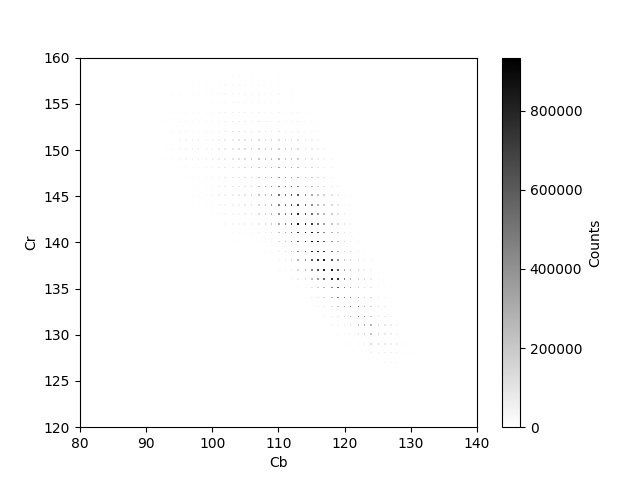
\includegraphics[width=.75\columnwidth]{histogram2d.png}
\caption{Cluster representando cor de pele na base SFA completa no espaço de cores CbCr}
\end{center}
\end{figure}

Há diversos algoritmos de classificação que podem ser usados, dos mais ingênuos e simplistas como por Limiarização até os mais sofisticados usado Redes Neurais, com diferentes custos-benefícios em termos de qualidade da segmentação versus tempo de execução.  

\subsection{Objetivos}
Neste projeto apresentaremos o resultado comparativo de custo-benefício de 3 métodos de deteção de pele: Por Limiarização, Classificador Bayesiano Simples e  K vizinhos mais próximos. A base de dados utilizada é a SFA\cite{sfa} criada especificamente para o problema de segementação de pele.

Mais especificamente deseja-se fazer:
\begin{enumerate}
\item  segmentação usando subconjunto da SFA (10 imagens);
\item  segmentação usando toda a base de imagens SFA (1118 imagens);
\item  análise dos resultados.
\end{enumerate}

\section{Revisão Teórica}

\subsection{Espaço de Cores}

Espaço de Cores é um modelo matemático que representa a informação de cor na forma de componentes, geralmente três ou quatro vetores. Por exemplo, o modelo RGB representa diferentes cores como uma composição de vermelho (R), verde (G) e azul (B). Diferentes modelos servem diferentes aplicações como computação gráfica, processamento de imagens, Transmissão de sinal de TV, entre outras. Alguns desses modelos são baseados em tonalidade (HSI, HSV e HSL) outros em Brilho (YCbCr, YIQ e YUV)\cite{kolkur}. 

\begin{figure}[ht!]
\begin{center}
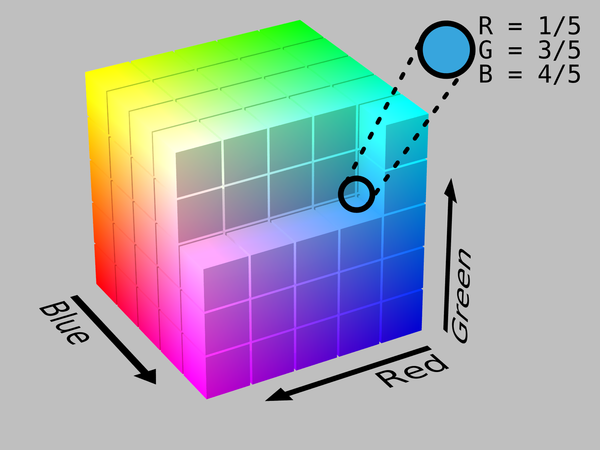
\includegraphics[width=.55\columnwidth]{RGB_Cube.png}
\caption{Modelo simplificado do espaço RGB\cite{wikipedia}}
\end{center}
\end{figure}

Apesar de nenhum modelo de espaço de cores ter sido criado especialmente para a aplicação de deteção de pele, os modelos baseados em brilho, como o YCbCr, facilitam a normalização proposta por \cite{yang}.

\subsection{Classificador baseado em Limiarização}
A classificação por limiarização (\textit{Threshold-based}) é um algoritmo muito simples e comumente encontrado em tutoriais de deteção de pele\cite{pysearch}. Em um determinado espaço de cor, definem-se limites mínimos e máximos da cor de pele, por exemplo:

\begin{equation}
\begin{split}
(R > 110) \cup(R < 210) \\
 \cup (G > 40) \cup (G < 100) \\
 \cup (B > 20) \cup (B < 60)
\end{split}
\end{equation}


O pixel que atende essa condição é classificado como \textit{pele}, os que não atendem como \textit{não-pele}. Apesar de simples, esse algoritmo tem a vantagem de ser potencialmente muito rápido, principalmente se não houver necessidade de transformação do espaço de cor da imagem.

Para escolher os limiares, pode-se usar sugestões publicadas em artigos ou gerar histogramas\ref{hists} para sua base de amostras e escolhê-los.

\begin{figure}
\label{hists}
\centering
\subfloat[R]{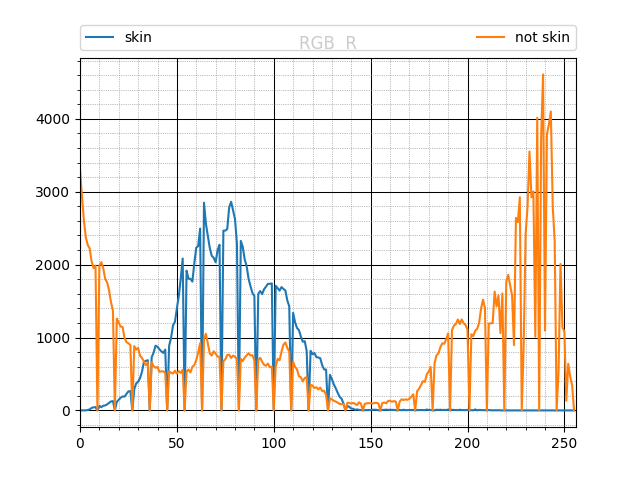
\includegraphics[width=2.6cm]{RGB-R.png}}\hfil
\subfloat[G]{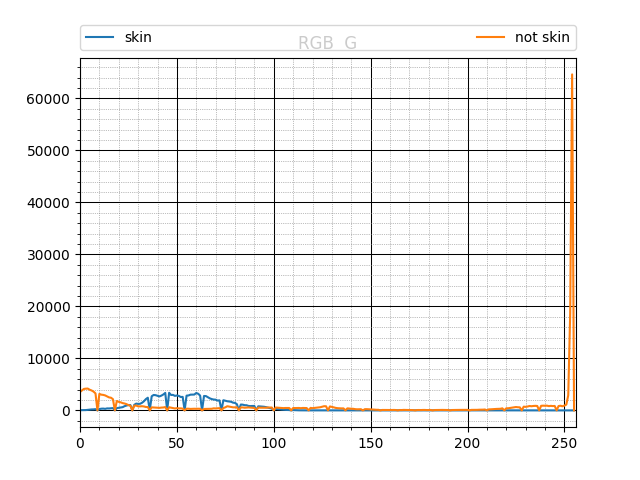
\includegraphics[width=2.6cm]{RGB-G.png}}\hfil 
\subfloat[B]{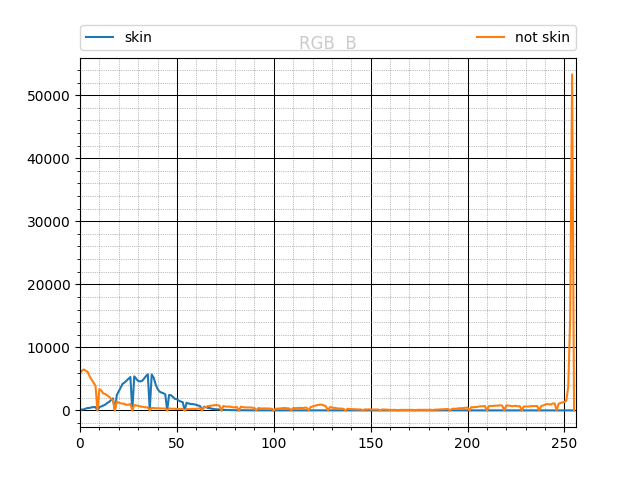
\includegraphics[width=2.6cm]{RGB-B.png}} 

\subfloat[Y]{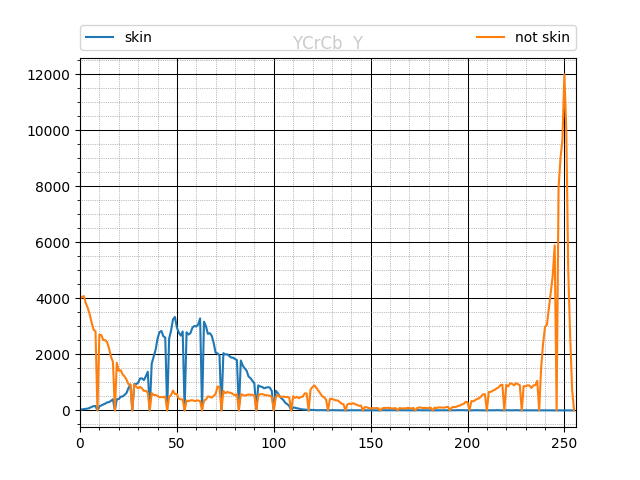
\includegraphics[width=2.6cm]{YCrCb-Y}}\hfil   
\subfloat[Cb]{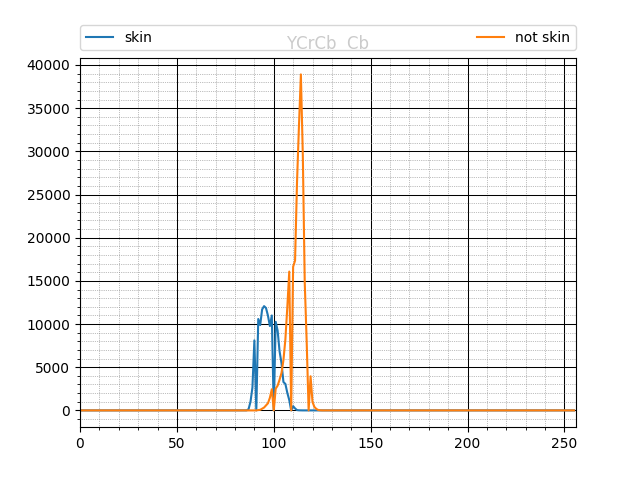
\includegraphics[width=2.6cm]{YCrCb-Cb}}\hfil
\subfloat[Cr]{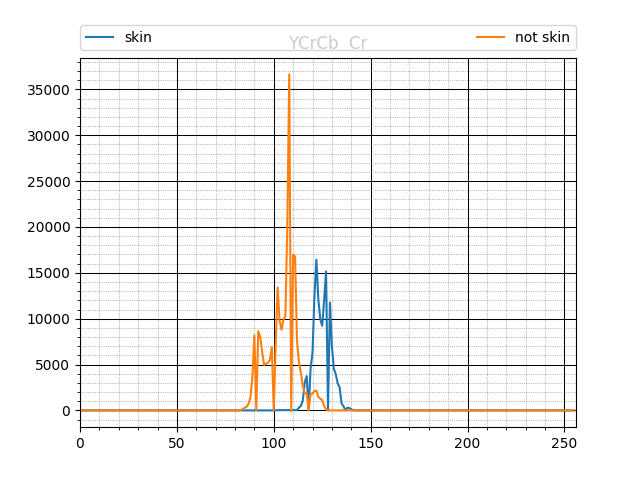
\includegraphics[width=2.6cm]{YCrCb-Cr}}
\caption{Histograma por canal dos pixels da base de treina- mento SFA reduzida}\label{figure}
\end{figure}

\subsection{Classificador Bayesiano Simples}
Em um Classificador Bayesiano Simples (ou Ingênuo), consideramos um conjunto de amostras classificadas em \textit{m} classes distintas \(C_1, C_2,...,C_m\), e \(X\) a tupla que se deseja classificar (não fazendo parte das amostras), o classificador encontra a classe \(C_i\) para o qual \(P(C_i \mid X)\) é a maior entre as classes existentes.

No nosso caso, temos só duas classes: \textit{pele} ou \textit{não-pele} (usaremos também os termos \textit{skin} ou \textit{background(bg)}); e, como usamos o espaço de cores YCbCr e normalizamos as imagens em relação ao brilho, simplesmente removendo o componente \(Y\), \(X\) é a tupla \(CbCr\), que aqui chamaremos de \(uv\).

Assim:
\begin{equation}
P(uv) = \frac{c[uv]}{T}
\end{equation}
onde \(c[uv]\) é a contagem de quantas vezes a tupla \(uv\) aparece nas amostras de treinamento e T é o total de pixels nas amostras. 

Para deteção de cor, usamos histogramas para determinar uma determinada probabilidade \(P(uv \mid skin)\) de um determinado valor \(CbCr\) ser da classe \textit{pele}. Tal probabilidade é obtida através do Teorema de Bayes\cite{teo}, onde a classe \textit{skin} é definida por:

$$ P(skin \mid uv) = \frac{P(uv \mid skin)P(skin)}{P(uv \mid skin) P(skin) + P(uv \mid bg) P(bg)} $$


$$P(skin) = \frac{T_s}{T}$$

\begin{equation}
P(uv \mid skin) = \frac{c_{skin}[uv]}{T_s}
\end{equation}
onde \(c_{skin}[uv]\) é a contagem de quantas vezes \(uv\) é classificado como \textit{skin} na base de treinamento e \(T_s\) é o total de pixels classificados como \textit{skin}. Os valores de \(P(bg)\) e \(P(uv \mid bg)\) podem ser obtidos da mesma forma.

Uma nova tupla /(uv) é classificada como \textit{pele} se:
$$P (skin \mid uv) > P (bg \mid uv)$$
que pode ser simplificado\cite{teo}:

$$c_{skin}[uv] > c_{bg}[uv]$$,


\subsection{K vizinhos mais próximos (K-NN)}

A classificação por K vizinhos mais próximos (K nearest neighbors - Knn) é o nome dado a uma família de técnicas usadas em problemas de classificação ou regressão\cite{goodfellow}. A priori, este classificador não exige uma fase de treinamento. Considerando um conjunto de amostras classificadas em \textit{m} classes distintas \(C_1, C_2,...,C_m\), e \(X\) a tupla que se deseja classificar (não fazendo parte das amostras), em tempo de execução o classificador encontra os K elementos conhecidos mais próximos de \(X\) e usa a classificação daqueles para definir a classe deste. 

Para definir proximidade, diferentes funções de distância podem ser utilizadas: euclidiana, manhattan, minkowski, ou até uma função personalizada para o problema. A classificação de K pode ser obtida através da média das classificações dos K vizinhos mais próximos, uma regra de votação (contagem) ou outra função personalizada ao problema.

Por ser um algoritmo genérico com alto potencial de aplicação, há diversas implementações disponíveis do mesmo. Neste projeto, usamos a implementação sklearn.neighbors da biblioteca SciPy\cite{scipy}


\begin{figure}[ht!]
\begin{center}
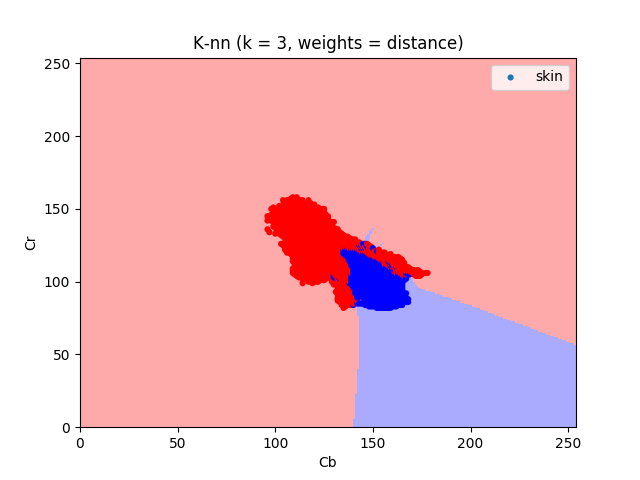
\includegraphics[width=\columnwidth]{knn-3.png}
\caption{Classificação 3-NN dos valores de Cb e Cr na base SFA reduzida.}
\end{center}
\end{figure}


\section{Metodologia}\label{metodologia}


\subsection{Materiais}
Foram utilizados:
\begin{itemize}
\item computador MacBook Pro (Retina, 13-inch, Early 2015), Processador Intel Core i5 2,7 GHz, 8GB de RAM
\item Python 3.6.3 :: Anaconda custom (64-bit)
\item OpenCV 3.4.0
\item dez programas em python especialmente desenvolvidos para o projeto. Todos estão disponíveis no repositório: \url{git@github.com:fredguth/unb-cv-3183.git}\label{repo}. Todos os tempos obtidos foram executados apenas usando apanas a CPU do computador.
\end{itemize}

\subsection{segmentação usando subconjunto da SFA (10 imagens)}
 \begin{enumerate}
  \item Executa-se o programa \textit{r1-a.py}, que gera o diretório \textit{results} uma série de histogramas de densidade de cores no \textit{dataset} em questão.
  \item Executa-se o programa \textit{r1-b.py}, que calcula o baseline para os parâmetros de acuidade e índice jaccard, através de um algoritmo nulo, que apenas classifica todos os pixels como \textit{não-pele} e anotam-se os resultados. 
  \item A partir dos histogramas, definem-se o espaço de cor apropriado e os limites que serão utilizados para cada canal de cor, inserindo-se no  programa \textit{r1-c.py}.
  \item Executa-se o programa \textit{r1-c.py}, que implementa um classificador por limiarização no espaço BGR muito simples, aplicando apenas um limite no canal azul e não faz nenhuma transformação no espaço de cores, e um classificador no espaço YCbCr que aplica limites aos canais Cb e Cr. Anotam-se os resultados.
  \item Executa-se o programa \textit{r1-d.py}, que implementa um classificador bayesisano simples e anotam-se os resultados.
   \item Executa-se o programa \textit{r1-e.py}, que implementa um classificador k-nn e anotam-se os resultados.
\end{enumerate}

\subsection{segmentação usando toda a base de imagens SFA (1118 imagens)}
 \begin{enumerate}
  \item Executa-se o programa \textit{r2-a.py}, que gera o diretório \textit{results} uma série de histogramas de densidade de cores no \textit{dataset} em questão.
  \item Executa-se o programa \textit{r2-b.py}, que calcula o baseline para os parâmetros de acuidade e índice jaccard, através do algoritmo nulo e anotam-se os resultados. 
  \item A partir dos histogramas, definem-se o espaço de cor apropriado e os limites que serão utilizados para cada canal de cor, inserindo-se no  programa \textit{r2-c.py}.
  \item Executa-se o programa \textit{r2-c.py}, que implementa um classificador por limiarização e anotam-se os resultados.
  \item Executa-se o programa \textit{r2-d.py}, que implementa um classificador bayesisano simples e anotam-se os resultados.
   \item Executa-se o programa \textit{r2-e.py}, que implementa um classificador k-nn e anotam-se os resultados.
\end{enumerate}


\section{Resultados}
Nesta seção apresentamos os resultados obtidos. Todos os dados podem ser acessados no repositório do projeto (\ref{repo}).
% \item  segmentação usando subconjunto da SFA (10 imagens);
% \item  segmentação usando toda a base de imagens SFA (1118 imagens);
% \item  análise dos resultados.
\subsection{Segmentação usando subconjunto da SFA (10 imagens)}
\begin{figure}[ht!]
\label{sfa10}
\begin{center}
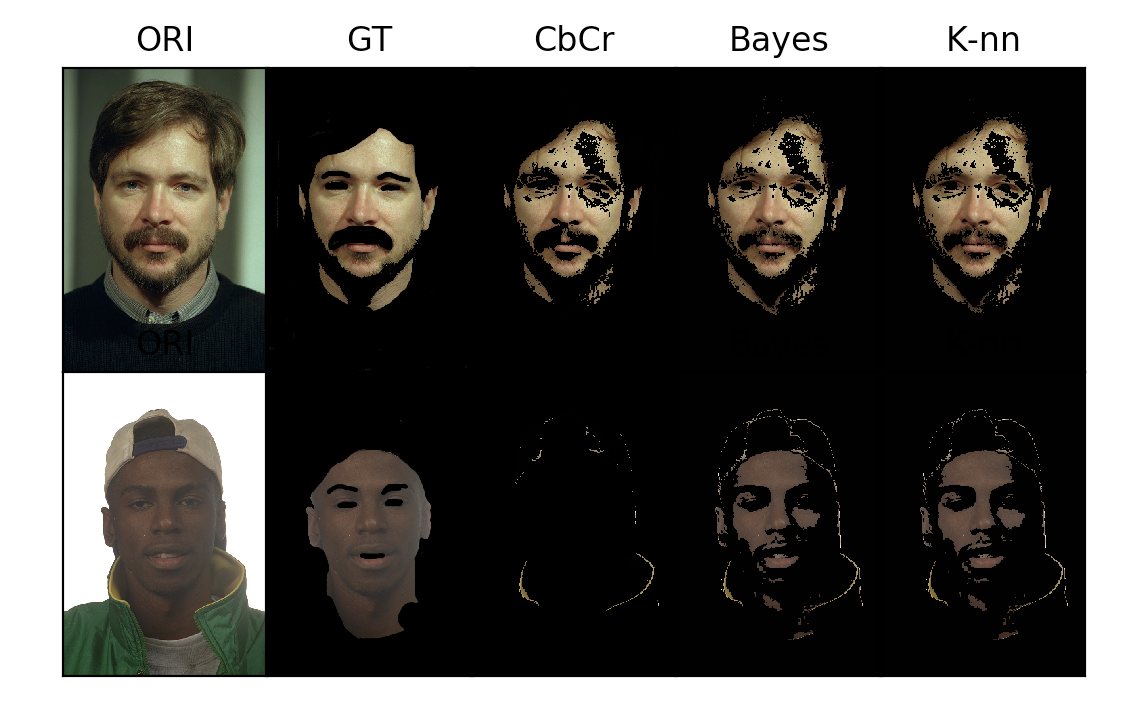
\includegraphics[width=\columnwidth]{sfa10.png}
\caption{Resultado qualitativo dos diferentes algoritmos.}
\end{center}
\end{figure}
O resultado qualitativo obtido com os diferentes algoritmos pode ser apreciado em \ref{sfa10}.



\begin{table}[]
\centering
\caption{Base SFA 10 imagens (8 treinamento, 2 teste)}
\label{table_sfa10}
\begin{tabular}{|r|c|c|c|c|}
\hline
\multicolumn{1}{|c|}{\multirow{2}{*}{Algoritmo}} & \multicolumn{2}{c|}{Qualidade} & \multicolumn{2}{c|}{Tempo Execução} \\ \cline{2-5} 
\multicolumn{1}{|c|}{} & Acuidade (\%) & Índice Jaccard (\%) & Treinamento (s) & Teste (s) \\ \hline
Nulo & 74.47 & 0.0 & 0 & 0 \\ \hline
Lim (B) & 44.41 & 11.11 & 0 & 0.06 \\ \hline
Lim(CbCr) & 81.15 & 34.37 & 0 & 0.04 \\ \hline
Bayes & 86.11 & 45.20 & 3.62 & 0.84 \\ \hline
K-nn & 84.97 & 45.64 & 3.46 & 8.59 \\ \hline
\end{tabular}
\end{table}
Para uma análise quantitativa da qualidade e do tempo de execução, temos \ref{table_sfa10}
\subsection{segmentação usando toda a base de imagens SFA (1118 imagens)}

\begin{figure}[ht!]
\label{sfa1118}
\begin{center}
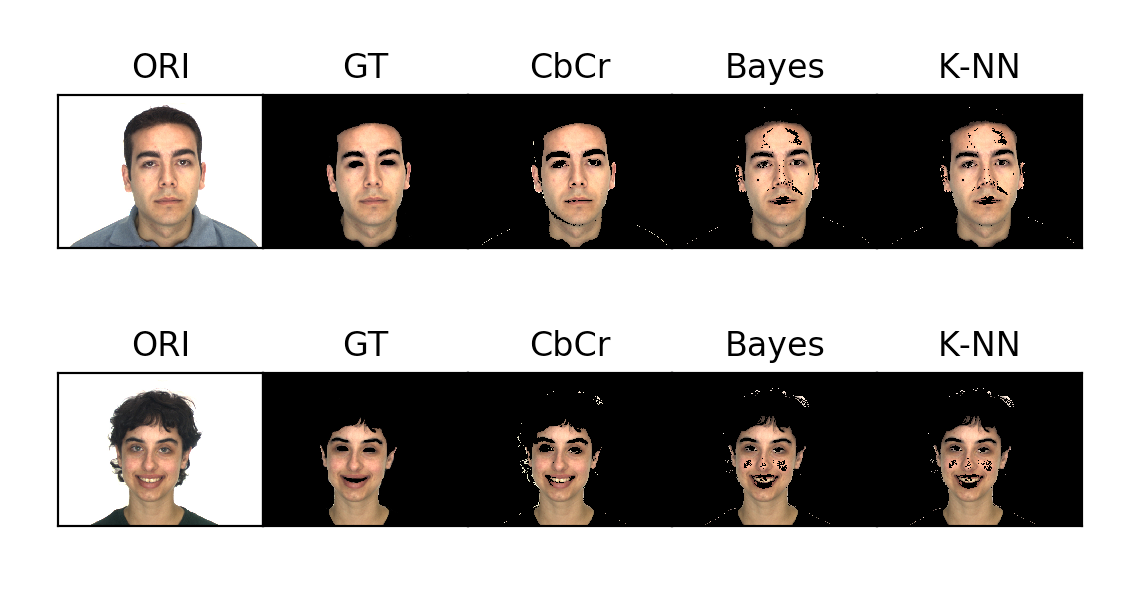
\includegraphics[width=\columnwidth]{sfa1118.png}
\caption{Resultado qualitativo dos diferentes algoritmos.}
\end{center}
\end{figure}
O resultado qualitativo obtido com os diferentes algoritmos pode ser apreciado em \ref{sfa1118}.

\begin{table}[]
\centering
\caption{Base SFA 1118 imagens\\ ( 782 treinamento, 167 validação, 167 teste)}
\label{table_sfa1118}
\begin{tabular}{|r|c|c|c|c|}
\hline
\multicolumn{1}{|c|}{\multirow{2}{*}{Algoritmo}} & \multicolumn{2}{c|}{Qualidade} & \multicolumn{2}{c|}{Tempo Execução} \\ \cline{2-5} 
\multicolumn{1}{|c|}{} & Acuidade (\%) & Jaccard (\%) & Trein. (s) & Teste (s) \\ \hline
Nulo & 79.59 & 0.0 & 0 & 0 \\ \hline
Lim (B) & 69.64 & 1.38 & 0 & 3.33\\ \hline
(CbCr) & 95.03 & 77.78 & 0 & 3.01 \\ \hline
Bayes & 94.62 & 76.77 & 364 & 77 \\ \hline
K-nn & 94.49 & 77.00 & 406 & 1660 \\ \hline
\end{tabular}
\end{table}
Para uma análise quantitativa da qualidade e do tempo de execução, temos \ref{table_sfa1118}
\subsection{Análise dos resultados}
Em face aos resultados obtidos, cabem algumas análises:
\begin{enumerate}
    \item O uso de um algoritmo nulo se mostrou muito importante, uma vez que apontou que a métrica escolhida como acuidade (pixels segmentados corretamente em relação ao total de pixels da imagem) é uma métrica muito ruim, uma vez que dado que as cores que representam pele são um pequeno cluster dentro do espaço de cores, \(P(bg)\) é muito maior, logo o algoritmo nulo consegue bons resultados de acuidade. 

    O índice Jaccard é melhor nesse sentido, mas não discrimina falsos positivos de falsos negativos.
    \item O algoritmo por limiarização CbCr apresentou um resultado quantitativo melhor do que o esperado. Já esperava-se que fosse rápido, e foi, classificando 167 imagens de teste em apenas 3 segundos. Há de se considerar o fator "sorte" na escolha dos limites para essa base. A análise qualitativa, entretanto, mostra que para amostras pequenas é razoavelmente pior do que o classificador bayesiano e o k-nn.
    \item A limirização apenas pelo canal B em RGB tinha pouca chance de ir bem e confirmou o que esperávamos. Mais interessante foi notar que a biblioteca OpenCV\cite{OpenCV} não apresenta nenhuma diferença de tempo para carregar imagens no espaço RGB (que é o mesmo da imagem de origem) e carregar no espaço YCbCr. 
    \item Os algoritmo bayesiano se mostrou uma alternativa mais robusta que o de limiarização, apresentando um resultado muito melhor na base pequena e bastante rápido também, levando 77 segundos para testar 167 imagens (menos de 0.5 segundo por imagem em uma CPU antiga).
\end{enumerate}


\section{Discussão e Conclusões}
Neste trabalho, implementamos três algoritmos para a segmentação de cor de pele em imagens e apresentamos os diferentes custos-benefícios.Demonstramos que, em conformidade com a teoria existente, a segmentação de pele por cor usando algoritmos simples de classificação atinge bons resultados que são mais do que suficiente para diversas aplicações de pré-processamento. 

% \begin{figure}[htbp]
% \centerline{
\includegraphics{fig.jpg}}
% \caption{Example of a figure caption.}
% \label{fig}
% \end{figure}

\selectlanguage{brazilian}
\bibliographystyle{IEEEtran}
\bibliography{references}

\end{document}
